\chapter{Априорное распределения параметров моделей машинного обучения}

Повышение точности аппроксимации в задачах машинного обучения влечет за собой повышение сложности моделей и как следствие снижает их интерпретируемость. Примером такого усложнения являются следующие модели: трансформеры~\cite{Vaswani2017}, BERT~\cite{Devlin2018}, ResNet~\cite{Kaiming2015} а также ансамбли этих моделей. 

При построении модели машинного обучения используется два свойства: сложность модели и точность аппроксимации модели. Сложность влияет на время, которое модель требуется для принятия решения, а также на интерпретируемость модели, следовательно модель которая имеют меньшую сложность является более предпочтительной~\cite{bachteev2018}. С другой стороны точность аппроксимации модели нужно максимизировать. В данной работе рассматривается метод \textit{дистилляции} модели. Данные метод позволяет строить новые модели на основе ранее обученых моделей.

\begin{definition}
Дистилляция модели --- снижение сложности модели путем выбора модели в множестве более простых моделей на основе параметров и ответов более сложной фиксированной модели.
\end{definition}

В работе~\cite{Hinton2015} Дж.\,Е. Хинтоном рассматривается метод дистилляции моделей машинного обучения для задачи классификации. В работе проведен ряд экспериментов, в которых проводилась дистилляции моделей для разных задач машинного обучения. Эксперимент на выборке MNIST~\cite{mnist}, в котором избыточно сложно нейросеть была дистиллирована в нейросеть меньшей сложности. Эксперимент по Speech Recognition, в котором ансамбль моделей был \textit{дистиллирован} в одну модель. Также в работе~\cite{Hinton2015} был проведен эксперимент по обучению экспертных моделей на основе одной большой модели.

\begin{definition}
Привилегированная информация --- множество признаков, которые доступны только в момент выбора модели, но не в момент тестирования.
\end{definition}

В работе~\cite{Vapnik2015} В.\,Н. Вапником введено понятия \textit{привилегированной информации}. В работе~\cite{Lopez2016} метод дистилляции~\cite{Hinton2015} используется вместе с привилегированным обучениям~\cite{Vapnik2015}. В предложенном методе на первом этапе обучается модель \textit{учителя} в пространстве привилегированной информации, после чего обучается модель \textit{ученика} в исходном признаковом пространстве используя \textit{дистилляцию}~\cite{Hinton2015}. Для обучения строится функция ошибки специального вида, анализируемая в данной работе. Эта функция состоит из нескольких слагаемых, включая ошибки учителя, ученика и регуляризирующие элементы.  Первые варианты подобной функции ошибки были предложены А.\,Г. Ивахненко~\cite{Ivakhnenko1994}.

\begin{definition}
Учитель --- фиксируемая модель, ответы которой используются при выборе модели ученика.
\end{definition}

\begin{definition}
Ученик --- модель, которая выбирается согласно какого-либо критерия.
\end{definition}

В данной работе предлагается рассмотреть вероятностный подход к решению задачи дистилляции модели и задачи привилегированного обучения. Подход обобщается на случай, когда привилегированная информация доступна не для всех объектов из обучающей выборки. В рамках вероятностного подхода предлагается анализ и обобщение функции ошибки~\cite{Hinton2015, Lopez2016}. Рассматриваются частные задачи классификации и регрессии~\cite{Ivakhnenko1994}.


В рамках вычислительного эксперимента анализируются методы использующие и не использующие модель учителя при обучение модели ученика. Для анализа используются реальные выборки для задачи классификации изображений FashionMNIST~\cite{fashionmnist} и для задачи классификации текстов Twitter Sentiment Analysis~\cite{twiter2013}. Выборка FashionMNIST использовалась вместо общепринятой выборки MNIST, так как последняя имеет приемлемое качество аппроксимации даже для линейного классификатора. Вычислительный эксперимент использует модели разной сложности: линейная модель, полносвязная нейронная сеть, сверточная нейронная сеть~\cite{LeCun1989}, модель Bi-LSTM~\cite{Schmidhuber1997} и модель BERT~\cite{Devlin2018}.

Исследуется проблема снижения числа обучаемых параметров моделей машинного обучения. Примерами таких моделей, с избыточным число параметров, являются AlexNet~\cite{Krizhevsky2012}, VGGNet~\cite{Simonyan2014}, ResNet~\cite{Kaiming2015}, BERT~\cite{Devlin2018, Vaswani2017}, mT5~\cite{Linting2021}, GPT3~\cite{Brown2020} и другие.
\begin{table}[h!]
\caption{Анализ роста числа параметров при развитии моделей глубокого обучения}
\label{tb:intro:1}
\begin{center}
\resizebox{\textwidth}{!}{
\begin{tabular}{|l|l|l|l|l|l|l|}
\hline
Название               & AlexNet     & VGGNet      & ResNet      & BERT     & mT5   & GPT3  \\ \hline
Год                          & 2012        & 2014        & 2015        & 2018     & 2020  & 2020  \\ \hline
Тип данных             & изображение & изображение & изображение & текст    & текст & текст \\ \hline
Число параметров, млрд & $0{,}06$    & $0{,}13$    & $0{,}06$    & $0{,}34$ & $13$  & $175$ \\ \hline
\end{tabular}
}
\end{center}
\end{table}
Табл. \ref{tb:intro:1} описывает глубокие модели машинного обучения.
Число параметров моделей машинного обучения с годами растет.
Это влечет снижение интерпретируемости моделей.
Данная проблема рассматривается в специальном классе задач по состязательным атакам (англ. adversarial attack)~\cite{Zheng2020}.
Большое число параметров требует больших вычислительных ресурсов.
Из-за этого данные модели не могут быть использованы в мобильных устройствах.
Для снижения числа параметров предложен метод дистилляции модели~\cite{Hinton2015, Vapnik2015, Lopez2016}.
Дистиллируемая модель с большим числом параметров называется \textit{учитель}, а модель получаемая путем дистилляции называется \textit{ученик}.
При оптимизации параметров модели ученика используется модель учителя с фиксированными параметрами.

Идея дистилляции предложена в работах Дж.\,Е. Хинтона и В.\,Н. Вапником~\cite{Hinton2015, Vapnik2015, Lopez2016}. В этих работах предлагается использовать ответы учителя в качестве целевой переменной для обучения модели ученика.
Поставлен ряд экспериментов, в которых проводилась дистилляция моделей для задачи классификации машинного обучения.
Базовый эксперимент на выборке MNIST~\cite{mnist} показал применимость метода для дистилляции избыточно сложной нейросетевой модели в нейросетевую модель меньшей сложности.
Эксперимент по дистилляции ансамбля моделей в одну модель для решения задачи распознания речи. Также в работе~\cite{Hinton2015} был проведен эксперимент по обучению экспертных моделей на основе одной модели с большим числом параметров при помощи предложенного метода дистилляции на ответах учителя.

В работе~\cite{Zehao2017} предложен метод передачи селективности нейронов (англ. neuron selectivity transfer) основаный на минимизации специальной функции потерь основаной на максимальном среднем отклонении (англ. maximum mean discrepancy) между выходами всех слоев модели учителя и ученика. Вычислительный эксперимент показал эффективность данного метода для задачи классификации изображений на примере выборок CIFAR~\cite{cifar10} и ImageNet~\cite{imagenet}.

В данной работе предлагается методы основанный на байесовском выводе.
В качестве априорного распределения параметров модели ученика предлагается использовать апостериорное распределение параметров модели учителя.
Решается задача сопоставления пространства параметров модели учителя и модели ученика.
Авторы предлагают подход, основаный на последовательном сопоставлении пространств параметров модели ученика и учителя. 
\begin{definition}
\label{def:structure}
Структура модели --- множество структурных параметров модели, которые задают вид суперпозиции.
\end{definition}
\begin{definition}
\label{def:sopos}
Сопоставление параметрических моделей --- изменение структуры модели (одной или нескольких моделей) в результате которого векторы параметров различных моделей лежат в одном пространстве.
\end{definition}
В результате сопоставления, параметры модели учителя и модели ученика лежат в одном пространстве.
Как следствие, в качестве априорного распределения параметров модели ученика выбирается апостериорное распределение параметров модели учителя.
В данной работе в качестве параметрических моделей рассматривается полносвязная нейронная сеть.
В качестве структурных параметров модели выбраны число слоев, а также размер каждого скрытого слоя.

В рамках предложенного метода сопоставления параметрических моделей не оговорен выбор порядка на множестве параметров модели учителя.
Для этого предлагается упорядочивать параметры модели учителя на основе их значимости.
Первый нейрон является наиболее значимым, а последний нейрон наименее значимым.
Порядок задается на основе отношения плотности распределения упорядочивваемого параметра к плотности распределения параметра в нуле~\cite{graves2011} или на основе метода Белсли~\cite{grabovoy2019}.
В рамках данной работы порядок на параметрах в рамках одного слоя задается случайный образом.

В рамках вычислительного эксперимента проводится теоретический анализ. Предложенный метод дистилляции анализируется на примере синтетической выборки, а также на реальной выборке FashionMnist~\cite{fashionmnist}.

Данная работа посвящена прореживанию структуры сети. Предлагается удалять наименее релевантные параметры модели. Под релевантностью~\cite{cun1990} подразумевается то, насколько параметр влияет на функцию ошибки. Малая релевантность указывает на то, что удаление этого параметра не влечет значимого изменения функции ошибки. Метод предлагает построение исходной избыточной сложности нейросети с большим количеством избыточных параметров. Для определения релевантности параметров предлагается оптимизацировать параметры и гиперпараметры в единой процедуре. Для удаления параметров предлагается использовать метод Белсли~\cite{neychev2016}.


В данной работе предлагается метод введения отношения порядка на множестве параметров сложных параметрических моделей, таких как нейросеть. Рассматривается порядок, заданный при помощи ковариационной матрицы градиентов функции ошибки по параметрам модели~\cite{Mandt2017}. В работе~\cite{Chunyan2016} предложен итерационный метод для поиска ковариационной матрицы градиентов. Данный итерационный метод интегрируется в градиентный метод оптимизации Adam~\cite{kingma2014}.

Множество параметров упорядочивается по возрастанию дисперсии: от параметра с минимальной дисперсией до параметра с максимальной дисперсией градиента функции ошибки по соответствующему параметру модели. Предполагается, что малая дисперсия градиента указывает на то, что соответствующий параметр можно зафиксировать.

Для задания порядка на множестве параметров при помощи ковариационной матрицы вводится предположение о том, что фиксация параметров происходит в момент, когда все параметры модели находятся в некоторой окрестности локального минимума функции ошибки. Данное условие накладывается для корректного использования итерационного метода поиска ковариационной матрицы градиентов.

Заданный порядок на множестве параметров модели используется для фиксации тех параметров модели, которые оказываются предстоящими с точки зрения заданного порядка. Сначала фиксируются те параметры, которые имеют минимальную дисперсию градиента в окрестности локального минимума функции ошибки.

Для анализа свойств предложенного метода задания порядка на множестве параметров проводился вычислительный эксперимент. В качестве моделей рассматривались модели различной структурной сложности: линейные модели, нейросетевые модели. Предложенный метод задания порядка сравнивается с методом, в котором порядок задан произвольным образом.

\section{Привилегированное обучение Вапника и дистилляция Хинтона}

% \section{Постановка задачи обучения с учителем: Хинтона и Вапника}
Задано множество объектов $\bm{\Omega}$ и множество целевых переменных $\mathbb{Y}$. Множество $\mathbb{Y}=\{1,\cdots,K\}$ для задачи классификации, где $K$ число классов, множество $\mathbb{Y}=\mathbb{R}$ для задачи регрессии.
Для каждого объекта из $\omega_i \in \bm{\Omega}$ задана целевая переменная $\mathbf{y}_i = \mathbf{y}\bigr(\omega_i\bigr)$. Множество целевых переменных для всех объектов обозначим $\mathbf{Y}$.
Для множества $\bm{\Omega}$ задано отображение в некоторое признаковое пространство $\mathbb{R}^{n}$:
\[
\label{eq:st:phi}
\begin{aligned}
\varphi:\bm{\Omega} \to \mathbb{R}^{n}, \quad \left|\bm{\Omega}\right| = m,
\end{aligned}
\]
где $n$ размерность признакового пространства, а $m$ количество объектов в множестве $\bm{\Omega}$. Отображение $\varphi$ отображает объект $\omega_i \in \bm{\Omega}$ в соответствующий ему вектор признаков $\mathbf{x}_i = \varphi(\omega_i)$.
Пусть для объектов $\bm{\Omega}^* \subset \bm{\Omega}$ задана привилегированная информация:
\[
\label{eq:st:phi*}
\begin{aligned}
\varphi^*:\bm{\Omega}^* \to \mathbb{R}^{n^*}, \quad \left|\bm{\Omega}^*\right| = m^*,
\end{aligned}
\]
где $m^* \leq m$ --- число объектов с привилегированной информацией, $n^*$ --- число признаков в пространстве привилегированной информации. Отображение $\varphi^*$ отображает объект $\omega_i \in \bm{\Omega^*}$ в соответствующий ему вектор признаков $\mathbf{x}^*_i = \varphi^*(\omega_i)$.

Множество индексов объектов, для которых известна привилегированная информация, обозначим $\mathcal{I}$:
\[
\label{eq:st:3}
\begin{aligned}
\mathcal{I} = \{1 \leq i \leq m | \text{для $i$-го объекта задана привилегированная информация}\},
\end{aligned}
\]
а множество индексов объектов, для которых не известна привилегированная информация, обозначим $\{1, \cdots, m\}\setminus \mathcal{I} = \bar{\mathcal{I}}$.

Пусть на множестве привилегированных признаков задана функция учителя $\mathbf{f}\bigr(\mathbf{x}^*\bigr)$:
\[
\label{eq:st:4}
\begin{aligned}
\mathbf{f}:\mathbb{R}^{n^*} \to \mathbb{Y}^*,
\end{aligned}
\]
где $\mathbb{Y}^*=\mathbb{Y}$ для задачи регрессии и $\mathbb{Y}^*$ является единичным симплексом $\mathcal{S}_K$ в пространстве размерности $K$ для задачи классификации. Модель учителя $\mathbf{f}$ ставит объекты $\mathbf{X}^*$ в соответствие объектам $\mathbf{S},$ то есть  $\mathbf{f}\bigr(\mathbf{x}^*_i\bigr)=\mathbf{s}_i$.

Требуется выбрать модель ученика $\mathbf{g}\bigr(\mathbf{x}\bigr)$ из множества:
\[
\label{eq:st:G}
\begin{aligned}
\mathfrak{G} = \left\{\mathbf{g}| \mathbf{g}:\mathbb{R}^{n} \to \mathbb{Y}^*\right\},
\end{aligned}
\]
например для задачи классификации множество $\mathfrak{G}$ может быть параметрическим семейством функций линейных моделей:
\[
\label{eq:st:G:lin:cl}
\begin{aligned}
\mathfrak{G}_\text{lin,cl} = \left\{\mathbf{g}\bigr(\mathbf{W}, \mathbf{x}\bigr)| \mathbf{g}\bigr(\mathbf{W}, \mathbf{x}\bigr) = \textbf{softmax}\bigr(\mathbf{W}\mathbf{x}\bigr), \quad \mathbf{W} \in \mathbb{R}^{n\times K}\right\}.
\end{aligned}
\]

Рассмотрим описание метода предложеного в работах~\cite{Hinton2015, Lopez2016}. В рамках данных работ предполагается, что для всех данных доступна привилегированная информация $\mathcal{I} = \{1, 2, \cdots, m\}$. В работе~\cite{Hinton2015} решается задача классификации вида:
\[
    \mathfrak{D} = \{\left(\mathbf{x}_i, y_i\right)\}_{i=1}^{m}, \qquad \mathbf{x}_i \in \mathbb{R}^{n}, \quad y_i \in \mathbb{Y}=\{1, \cdots, K\},
\]
где $y_i$ --- это класс объекта, также будем обозначать $\mathbf{y}_i$ вектором вероятности для класса $y_i$.

В постановке Хинтона рассматривается параметрическое семейство функций:
\[
\label{eq:G:set:cl}
\mathfrak{G}_{\text{cl}} = \left\{\mathbf{g}| \mathbf{g} = \text{softmax}\bigr(\mathbf{z}\bigr(\mathbf{x}\bigr)/T\bigr), \quad \mathbf{z}: \mathbb{R}^n \to \mathbb{R}^K \right\},
\]
где $\mathbf{z}$ --- это дифференцируемая параметрическая функция заданной структуры, $T$ --- параметр температуры. В качестве модели учителя $\mathbf{f}$ рассматривается функция из множества $\mathfrak{F}_{\text{cl}}$:
\[
\label{eq:F:set:cl}
\mathfrak{F}_{\text{cl}} = \left\{\mathbf{f}| \mathbf{f} = \text{softmax}\bigr(\mathbf{v}\bigr(\mathbf{x}\bigr)/T\bigr), \quad \mathbf{v}: \mathbb{R}^n \to \mathbb{R}^K \right\},
\]
где $\mathbf{v}$ --- это дифференцируемая параметрическая функция заданной структуры, $T$ --- параметр температуры.
Параметр температуры $T$ имеет следующие свойства:
\begin{enumerate}
    \item при $T\to 0$ получаем вектор, в котором один из классов имеет единичную вероятность;
    \item при $T\to \infty$ получаем равновероятные классы.
\end{enumerate}

Функция потерь $\mathcal{L}$ в которой учитывается перенос информации от модели учителя $\mathbf{f}$ к модели ученика $\mathbf{g}$ имеет следующий вид:
\[
\label{eq:hinton:1}
\begin{aligned}
   \mathcal{L}_{st}\bigr(\mathbf{g}\bigr) = &-\sum_{i=1}^{m}\underbrace{{\sum_{k=1}^{K}y^k_i\log\mathbf{g}\bigr(\mathbf{x}_i\bigr)\bigr|_{T=1}}}_{\text{исходная функция потерь}}\\
   &-\sum_{i=1}^{m}\underbrace{{\sum_{k=1}^{K}\mathbf{f}\bigr(\mathbf{x}_i\bigr)\bigr|_{T=T_0}\log\mathbf{g}\bigr(\mathbf{x}_i\bigr)\bigr|_{T=T_0}}}_{\text{слагаемое дистилляция}},
\end{aligned}
\]
где $\cdot\bigr|_{T=t}$ обозначает, что параметр температуры $T$ в предыдущей функции равняется $t$.

Получаем оптимизационную задачу:
\[
\label{eq:hinton:opt}
\begin{aligned}
   \hat{\mathbf{g}} = \arg\min_{\mathbf{g} \in \mathfrak{G}_{\text{cl}}} \mathcal{L}_{st}\bigr(\mathbf{g}\bigr).
\end{aligned}
\]

Работа~\cite{Lopez2016} обобщает метод предложенный в работе~\cite{Hinton2015}. Решение задачи оптимизации \eqref{eq:hinton:opt} зависит только от вектора ответов модели учителя $\mathbf{f}$. Следовательно признаковые пространства учителя и ученика могут различаться. В этом случае получаем следующую постановку задачи:
\[
    \mathcal{D} = \left\{\left(\mathbf{x}_i, \mathbf{x}^*_i, y_i\right)\right\}_{i=1}^{m}, \qquad \mathbf{x}_i \in \mathbb{R}^{n}, \quad \mathbf{x}^*_i \in \mathbb{R}^{n^*}, \quad y_i \in \{1, \cdots, K\},
\]
где $\mathbf{x}_i$ это информация доступна на этапах обучения и контроля, а $\mathbf{x}^*_i$ это информация доступна только на этапе обучения. Модель учителя принадлежит множеству моделей $\mathfrak{F}_{cl}^*$:
\[
\label{eq:F:set:cl:priv}
\mathfrak{F}_{\text{cl}}^* = \left\{\mathbf{f}| \mathbf{f} = \text{softmax}\bigr(\mathbf{v}^*\bigr(\mathbf{x}^*\bigr)/T\bigr), \quad \mathbf{v}^*: \mathbb{R}^{n^*} \to \mathbb{R}^K \right\},
\]
где $\mathbf{v}^*$ --- это дифференцируемая параметрическая функция заданной структуры, $T$ --- параметр температуры. Множество моделей $\mathfrak{F}_{cl}^*$ отличается от множества моделей $\mathfrak{F}_{cl}$ из выражения \eqref{eq:F:set:cl}. В множестве $\mathfrak{F}_{cl}$ модели используют пространство исходных признаков, а в множестве $\mathfrak{F}_{cl}^*$ модели используют пространство привилегированных признаков. Функция потерь \eqref{eq:hinton:1} в случае модели учителя $\mathbf{f} \in \mathfrak{F}_{cl}^*$ переписывается в следующем виде:
\[
\label{eq:hinton:L:new}
\begin{aligned}
   \mathcal{L}_{st}\bigr(\mathbf{g}\bigr) = &-\sum_{i=1}^{m}{\sum_{k=1}^{K}y^k_i\log\mathbf{g}\bigr(\mathbf{x}_i\bigr)\bigr|_{T=1}}-\sum_{i=1}^{m}{\sum_{k=1}^{K}\mathbf{f}\bigr(\mathbf{x}^*_i\bigr)\bigr|_{T=T_0}\log\mathbf{g}\bigr(\mathbf{x}_i\bigr)\bigr|_{T=T_0}},
\end{aligned}
\]
где $\cdot\bigr|_{T=t}$ обозначает, что параметр температуры $T$ в предыдущей функции равняется $t$.

Требуется построить модель, которая использует привилегированную информацию $\mathbf{x}^*_i$ при обучении. Для этого рассмотрим двухэтапную модель обучения предложенную в работе~\cite{Lopez2016}:
\begin{enumerate}
    \item выбираем оптимальную модель учителя $\mathbf{f} \in \mathfrak{F}_{\text{cl}}^*$;
    \item выбираем оптимальную модель ученика $\mathbf{g} \in \mathfrak{G}_{\text{cl}}$ используя дистилляцию~\cite{Hinton2015}. 
\end{enumerate}

Модель ученика --- это функция, которая минимизирует \eqref{eq:hinton:L:new}. Модель учителя --- это функция, которая минимизирует кросс--энтропийную функции ошибки:
\[
\label{eq:hinton.2}
\begin{aligned}
   \mathcal{L}_{th}\bigr(\mathbf{f}\bigr) = &-\sum_{i=1}^{m}{{\sum_{k=1}^{K}y^k_i\log\mathbf{f}\bigr(\mathbf{x}^*_i\bigr)}}.
   \end{aligned}
\]

\section{Назначения релевантности параметров моделей}

Задана выборка
\[
\label{2.1}
\mathfrak{D} = \{\textbf{x}_i,y_i\},  i =1,...,N,
\]
где $\textbf{x}_i \in \mathbb{R}^{m}$, $y_i \in \{1, \dots, Y\}$, $Y$ --- число классов.
Рассмотрим модель $f(\mathbf{x}, \mathbf{w}): \mathbb{R}^m \times \mathbb{R}^n \to \{1,\dots,Y\}$, где $\textbf{w} \in \mathbb{R}^n$ --- пространство параметров модели,

\[
\label{2.2}
f(\mathbf{x}, \mathbf{w}) = \text{softmax}\bigl( f_1(f_2(...(f_l(\mathbf{x}, \mathbf{w})\bigr),
\]
где $f_i(\mathbf{x}, \mathbf{w}) =  \text{tanh}(\mathbf{w}^\mathsf{T}\mathbf{x})$, $l$ --- число слоев нейронной сети, $i \in \{1\dots l\}$.
Параметр $w_j$ модели $f$  называется активным, если $w_j \not = 0$. Множество индексов активных параметров обозначим $\mathcal{A} \subset \mathcal{J} = \{1,...,n\}$.
Задано пространство параметров модели:

\[
\label{2.3}
\mathbb{W_\mathcal{A}} = \{ \textbf{w} \in \mathbb{R}^n | w_j\not=0, j \in \mathcal{A}  \},
\]


Для модели $f$ с множеством индексов активных параметров $\mathcal{A}$ и соответствующего ей вектора параметров $\textbf{w} \in \mathbb{W_\mathcal{A}}$  определим логарифмическую функцию правдоподобия выборки:
\[
\label{2.4}
\mathcal{L}_\mathfrak{D}(\mathfrak{D}, \mathcal{A}, \textbf{w}) = \log p(\mathfrak{D}|\mathcal{A}, \textbf{w}),
\]
где $p(\mathfrak{D}|\mathcal{A},\textbf{w})$ --- апостериорная вероятность выборки $\mathfrak{D}$ при заданных $\textbf{w}, \mathcal{A}$.
Оптимальные значения $\textbf{w},\mathcal{A}$ находятся из минимизации $-\mathcal{L}_{\mathcal{A}}(\mathfrak{D},\mathcal{A})$ --- логарифма правдоподобия модели:
\[
\label{2.5}
\mathcal{L}_{\mathcal{A}}(\mathfrak{D},\mathcal{A}) =\log p(\mathfrak{D}|\mathcal{A}) = \log  \int_{{\textbf{w}\in\mathbb{W_\mathcal{J}}}}
p(\mathfrak{D} | \textbf{w}) p(\textbf{w} | \mathcal{A}) d \textbf{w},
\]
где $p(\textbf{w}|\mathcal{A})$ ---  априорная вероятность вектора параметров в пространстве $\mathbb{W_\mathcal{J}}$.

Так как вычисление интеграла \eqref{2.5} является вычислительно сложной задачей, рассмотрим вариационный подход~\cite{bishop2006} для решения этой задачи. Пусть задано распределение $q$:
\[
\label{2.6}
q(\textbf{w})\sim \mathcal{N}(\textbf{m}, \textbf{A}^{-1}_\text{ps}),
\]
где $\textbf{m}, \textbf{A}^{-1}_\text{ps}$ --- вектор средних и матрица ковариации, аппроксимирующее неизвестное апостериорное распределение $p(\textbf{w}|\mathfrak{D},\mathcal{A})$:
\[
\label{2.7}
p(\textbf{w} | \mathcal{A})\sim \mathcal{N}(\boldsymbol{\mu},\textbf{A}^{-1}_{\text{pr}}),
\]
где $\boldsymbol{\mu},\textbf{A}^{-1}_{\text{pr}}$ --- вектор средних и матрица ковариации.

Приблизим интеграл \eqref{2.5} методом из~\cite{bishop2006}:

\[
\label{2.8}
\begin{aligned}
\mathcal{L}_{\mathcal{A}}(\mathfrak{D},\mathcal{A}) = \log p(\mathfrak{D}|\mathcal{A}) = \\
=\int_{\textbf{w}\in\mathbb{W_\mathcal{J}}} q(\textbf{w}) \log \frac{p(\mathfrak{D}, \textbf{w}|\mathcal{A})}{q(\textbf{w})}d \textbf{w} - \int_{\textbf{w}\in\mathbb{W_\mathcal{J}}}  q(\textbf{w}) \log \frac{p(\textbf{w}|\mathfrak{D},\mathcal{A})}{q(\textbf{w})}d \textbf{w} \approx \\
\approx \int_{\textbf{w}\in\mathbb{W_\mathcal{J}}} q(\textbf{w}) \log \frac{p(\mathfrak{D}, \textbf{w}|\mathcal{A})}{q(\textbf{w})}d \textbf{w} = \\
= \int_{\textbf{w}\in\mathbb{W_\mathcal{J}}} q(\textbf{w}) \log \frac{p(\textbf{w}| \mathcal{A})}{q(\textbf{w})}d \textbf{w} + \int_{\textbf{w}\in\mathbb{W_\mathcal{J}}} q(\textbf{w}) \log p(\mathfrak{D}|\mathcal{A}, \textbf{w})d \textbf{w}=\\
=\mathcal{L}_\textbf{w}(\mathfrak{D}, \mathcal{A}, \textbf{w})+\mathcal{L}_{E}(\mathfrak{D},\mathcal{A}).
\end{aligned}
\]

Первое слагаемое формулы \eqref{2.8} --- это сложность модели. Оно определяется расстоянием Кульбака-Лейблера:
\[
\label{2.9}
\mathcal{L}_\textbf{w}(\mathfrak{D}, \mathcal{A}, \textbf{w}) = -D_{KL}\bigl(q(\textbf{w})||p(\textbf{w}|\mathcal{A})\bigr).
\]
Второе слагаемое формулы \eqref{2.8} является матожиданием правдоподобия выборки $\mathcal{L}_\mathfrak{D}(\mathfrak{D},\mathcal{A}, \textbf{w})$. В данной работе оно является функцией ошибки:
\[
\label{2.10}
\mathcal{L}_{E}(\mathfrak{D},\mathcal{A}) = \mathsf{E}_{\textbf{w}\sim q}\mathcal{L}_\mathfrak{D}(\textbf{y}, \mathfrak{D}, \mathcal{A}, \textbf{w}).
\]

Требуется найти параметры, доcтавляющие минимум суммарному функционалу потерь $\mathcal{L}_\mathcal{A}(\mathfrak{D},\mathcal{A},\textbf{w})$ из \eqref{2.8}:
\[
\label{2.11}
\begin{aligned}
\hat{\textbf{w}} = \arg\min_{\mathcal{A}\subset\mathcal{J}, \textbf{w} \in \mathbb{W_\mathcal{A}}} -\mathcal{L}_\mathcal{A}(\mathfrak{D}, \mathcal{A}, \textbf{w}) = 
=\arg\min_{\mathcal{A}\subset\mathcal{J}, \textbf{w} \in \mathbb{W_\mathcal{A}}} D_{KL}\bigl(q(\textbf{w})||p(\textbf{w}|\mathcal{A})\bigr) - \mathcal{L}_\mathfrak{D}(\mathfrak{D}, \mathcal{A}, \textbf{w}).
\end{aligned}
\]

\paragraph{Случайное удаление.}
Метод случайного удаления заключается в том, что случайным образом удаляется некоторый параметр $w_\xi$ из множества активных параметров сети.  Индекс параметра $\xi$ из равномерного распределения  случайная величина, предположительно доставляющая оптимум в \eqref{2.11}.
\[
\label{3.1.1}
\xi \sim \mathcal{U}(\mathcal{A}).
\]

\paragraph{Оптимальное прореживание.}
Метод оптимального прореживания~\cite{cun1990} использует вторую производную целевой функции \eqref{2.4} по параметрам для определения нерелевантных параметров. Рассмотрим функцию потерь $\mathcal{L}$ \eqref{2.4} разложенную в ряд Тейлора в некоторой окрестности вектора параметров $\textbf{w}$:
\[
\label{3.2.1}
\delta \mathcal{L} = \sum_{j\in \mathcal{A}} g_j\delta w_j + \frac{1}{2}\sum_{i,j\in \mathcal{A}} h_{ij}\delta w_i\delta w_j + O(||\delta\textbf{w}||^3),
\]
где $\delta w_j $ --- компоненты вектора $\delta\textbf{w}$, $g_j$ --- компоненты вектора градиента $\nabla \mathcal{L}$, а $h_{ij}$ --- компоненты гесcиана $\textbf{H}$:
\[
\label{3.2.2}
g_j = \frac{\partial \mathcal{L}}{\partial w_j}, \qquad h_{ij} = \frac{\partial^2\mathcal{L}}{\partial w_i \partial w_j}.
\]

Задача является вычислительно сложной в силу размерности матрицы \textbf{H}. Введем следующее предположение~\cite{cun1990}, о том что удаление нескольких параметров приводит к такому же изменению функции потерь $\mathcal{L}$, как и суммарное изменение при индивидуальном удалении:
\[
\label{3.2.3}
\delta \mathcal{L} = \sum_{j\in \mathcal{A}} \delta \mathcal{L}_j,
\]
где $\mathcal{A}$ --- множество активных параметров, $\delta\mathcal{L}_j$ --- изменение функции потерь, при удалении одного параметра $\textbf{w}_j$.

В силу данного предположения будем рассматривать только диагональные элементы матрицы \textbf{H}. После введенного предположения, выражение \eqref{3.2.1} принимает вид
\[
\label{3.2.4}
\delta \mathcal{L} = \frac{1}{2} \sum_{j\in \mathcal{A}} h_{jj}\delta w_j^2, 
\]

Получаем следующую задачу оптимизации:

\[
\label{3.2.5}
\xi = \arg\min_{j\in \mathcal{A}} h_{jj}\frac{w_j^2}{2},
\]
где $\xi$ --- индекс наименее релевантного, удаляемого параметра, предположительно доставляющая оптимум в \eqref{2.11}.

\paragraph{Удаление неинформативных параметров с помощью вариационного вывода.}
Для удаления параметров в работе~\cite{graves2011} предлагается удалить параметры, которые имеют максимальное отношение плотности $p(\textbf{w}|\mathcal{A})$ априорной вероятности в нуле к плотности вероятности априорной вероятности в математическом ожидании параметра.\\
Для гауссовского распределения с диагональной матрицей ковариации получаем:
\[
\label{3.3.1}
p_j(\textbf{w}|\mathcal{A})(x) = \frac{1}{\sqrt[]{2\sigma_j^2}}\exp({-\frac{(x-\mu_j)^2}{2\sigma_j^2}}).
\]
Разделив плотность вероятности в нуле к плотности в математическом ожидание
\[
\label{3.3.2}
\frac{p_j(\textbf{w}|\mathcal{A})(0)}{p_j(\textbf{w}|\mathcal{A})(\mu_j)}= \exp({-\frac{\mu_j^2}{2\sigma_j^2}}),
\]
Получаем следующую задачу оптимизации:
\[
\label{3.3.3}
\xi = \arg\min_{j\in \mathcal{A}} \left|\frac{\mu_j}{\sigma_j}\right|,
\]
где $\xi$ --- индекс наименее релевантного, удаляемого параметра.

\section{Смесь экспертов для аппроксимации мультимодальной выборки }

В статье исследуется проблема построения смеси экспертов.
Смесь экспертов - это мультимодель, которая состоит из множества локальных моделей, которые называются экспертами и шлюзовой функции.
Смест экспертов использует шлюзовую функцию для взвешивания прогнозов каждого эксперта.
Весовые коэффициенты шлюзовую функции зависят от объекта, для которого производится прогноз.
Примерами мультимоделей являются бэггинг,  градиентный бустинг~\cite{Tianqi2016} и случайный лес~\cite{Ishwaran2012}.
В статье~\cite{Yuksel2012} предполагается, что вклад каждого эксперта в ответ зависит от объекта из набора данных.

Основной проблемой построения мультимоделей является то, что ансамбль зависит от начальной инициализации параметров. Для улучшения устойчивости мультимодели предлагается использовать вероятностную постановку задачи для поиска оптимальных параметров шлюзовой функции и параметров локальной модели. В данной работе задается априорное распределения на параметры локальных моделей, также, для повышения, предлагается учесть зависимость априорных распределений для разных моделей.

\begin{figure}[h!t]\center
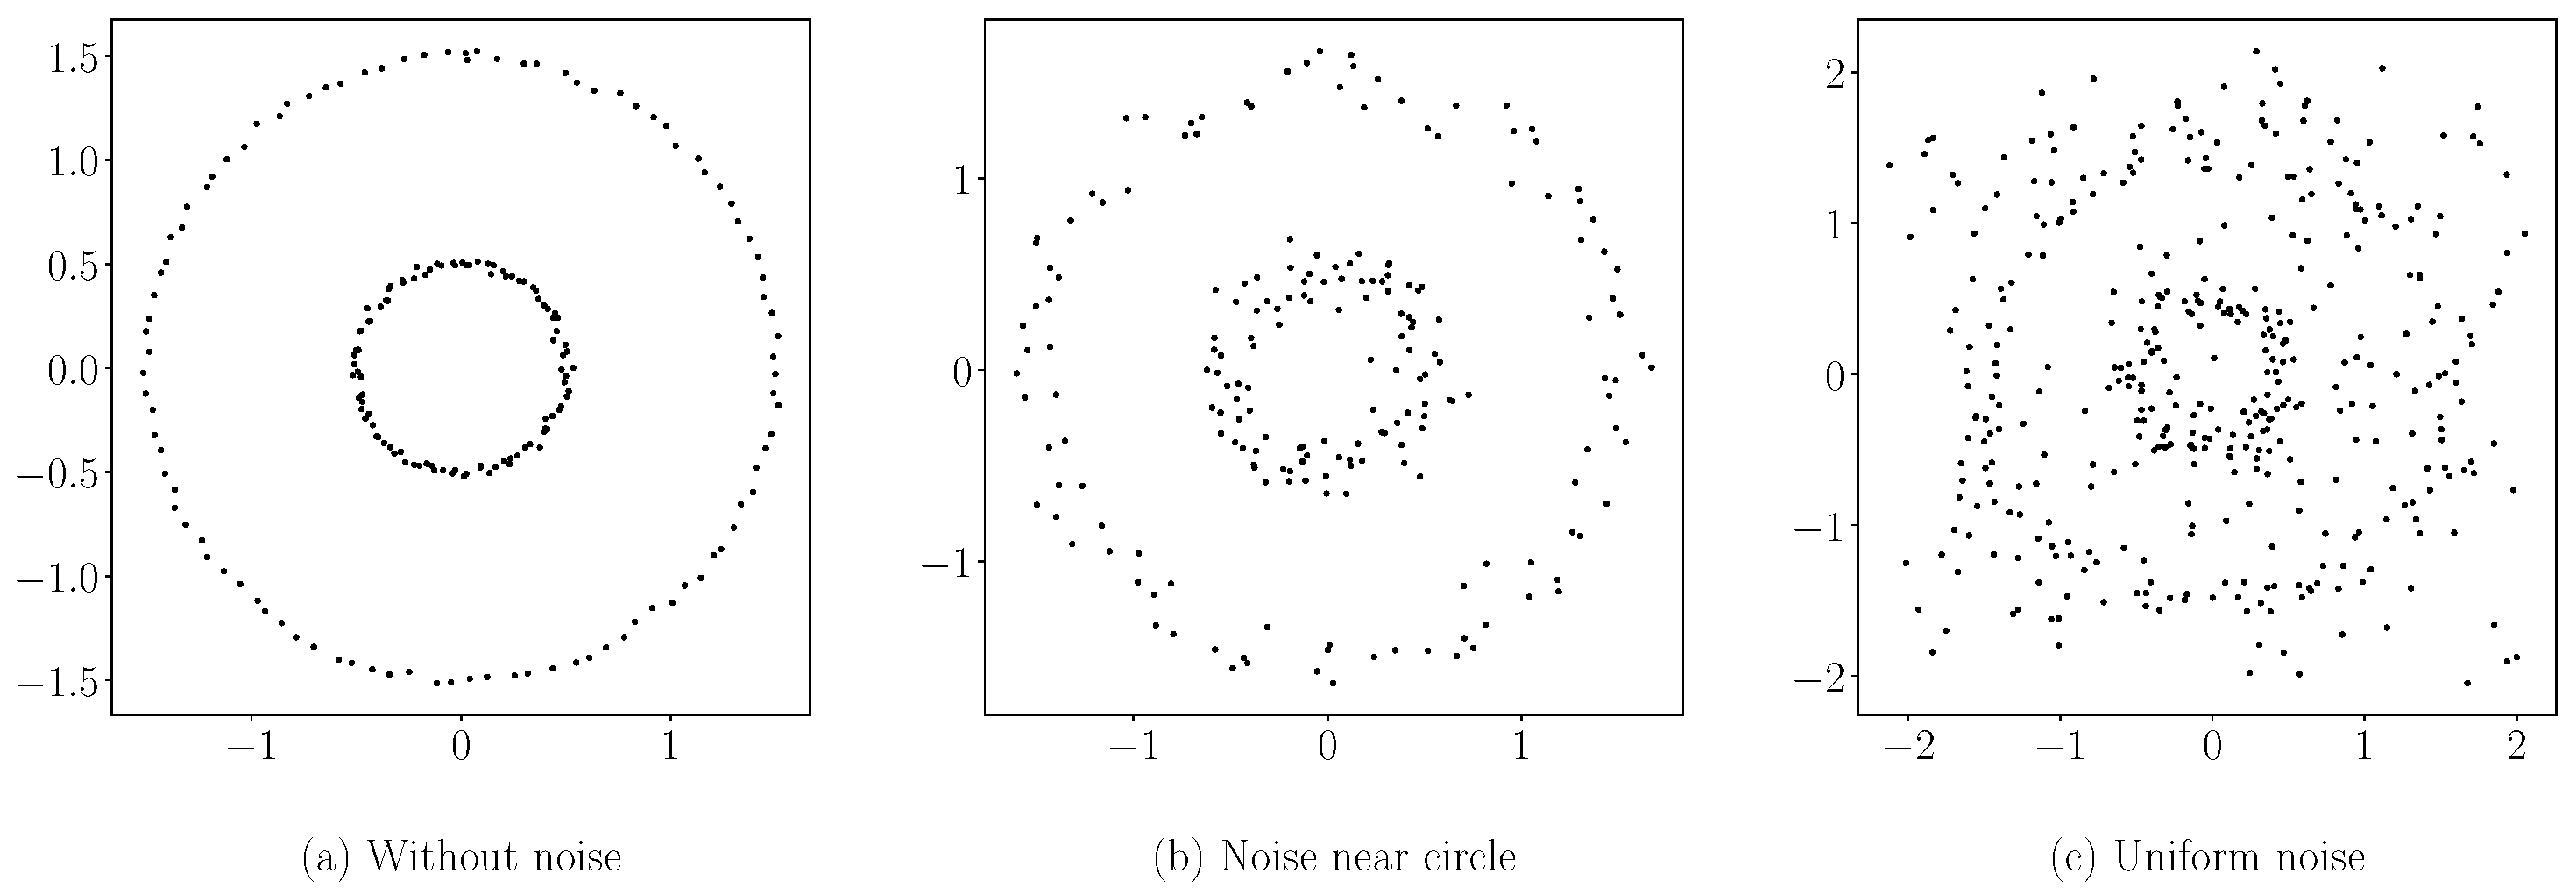
\includegraphics[width=1\textwidth]{results/priorexpert/statment}
\caption{Пример окружностей с разным уровнем шума: (a) окружности без шума; (b) окружности с зашумленным радиусом; (c) окружности с зашумленным радиусом, а также с равномерным шумом по всему изображению}
\label{example:1}
\end{figure}

В данной работе решается задача поиска окружностей на бинаризованном изображении. Предполагается, что радиусы окружностей различаются значимо, а также, что центры почти совпадают. Пример изображений показан на рис. \ref{example:1}. В данной работе в качестве экспертов рассматриваются линейные модели --- каждая модель аппроксимирует одну окружности. В качестве шлюзовой функции рассматривается двухслойная нейронная сеть.

Большое количество работ в области построения смеси экспертов посвящены выбору шлюзовой функции: используется softmax, процесс Дирихле~\cite{Edward2002}, нейронная сеть~\cite{Shazeer2017} с функцией softmax на последнем слое. Ряд работ посвящены выбору моделей в качестве отдельных экспертов. В работах~\cite{Jordan1994, Jordan1991} в качестве модели эксперта рассматривается линейная модель. Работы~\cite{Lima2007, Cao2003} рассматриваю модель SVM в качестве модели эксперта.
В работе~\cite{Yuksel2012} представлен обзор методов и моделей в задачах смеси экспертов.

Смесь экспертов имеет множество приложений в прикладных задачах. Работы~\cite{Yumlu2003, Cheung1995, Weigend2000} посвящены применению смеси экспертов в задачах прогнозирования временных рядов. 
В работе~\cite{Ebrahimpour2009} предложен метод распознавания рукописных цифр. 
Метод распознания текстов при помощи смеси экспертов иследуется в работах~\cite{Estabrooks2001}, распознание речи~\cite{Mossavat2010, Peng1996, Tuerk2001}. 
В работе~\cite{Sminchisescu2007} исследуется смесь экспертов для задачи распознавания трехмерных движений человека. 
В~\cite{Bowyer2010} описаны работы по исследованию обнаружения радужки глаза на изображении. В работах~\cite{Matveev2010, Matveev2014} в частности описаны методы выделения границ радужки и зрачка.

Построение интерпретируемых моделей в машинном обучении (Ribeiro et al. 2016) является одной из ключевых задач в машинном обучении.
Современные решения проблемы классификации изображений на основе сетей глубокого обучения ResNet, VGG, Intercept (Kaiming et al., 2016) являются плохо интерпретируемыми моделями.
В работах (Han et al. 2020; Akhtar et al. 2018)  показано, что сети глубокого обучения чувствительны даже к небольшому шуму в данных, что связано с их неинтерпретируемостью.

В этом разделе мы предлагаем метод \textit{обучения с экспертом}.
Этот метод предполагает использование предметных знаний экспертов для улучшения качества аппроксимации, а также для получения интерпретируемых моделей машинного обучения.
Предметные знания экспертов об образце будут называться \textit{экспертная информация}.
Предполагается, что использование экспертной информации позволяет аппроксимировать выборку простыми интерпретируемыми моделями, такими как линейные модели. Методы машинного обучения, которые учитывают экспертные знания при построении моделей, называются \textit{экспертным обучением}.


В статье решается задача аппроксимации кривых второго порядка на контурном изображении. Кривые второго порядка выбираются для анализа, так как они легко описываются линейными моделями. В этом случае эти фигуры необходимо восстанавливать в таких прикладных задачах, как задача распознавания радужной оболочки глаза (Matveev 2010; Matveev et al. 2014; Bowyer et al. 2010), задача описания трека частицы в адронный коллайдер (Salamani et al. 2018). Экспертная информация о кривой второго порядка позволяет отображать точки на плоскости в новое описание объекта, где каждая кривая аппроксимируется одной линейной моделью. Модель, которая аппроксимирует одну кривую, называется \textit{локальной моделью}. Для аппроксимации всего контурного изображения необходимо аппроксимировать несколько кривых второго порядка с помощью нескольких локальных моделей. В этой статье вводятся следующие ограничения на изображения: а) изображение состоит только из кривых второго порядка; б) изображение аппроксимируется небольшим количеством кривых второго порядка; в) количество и тип кривых на изображении известны.

\begin{figure}[h!]
\center
     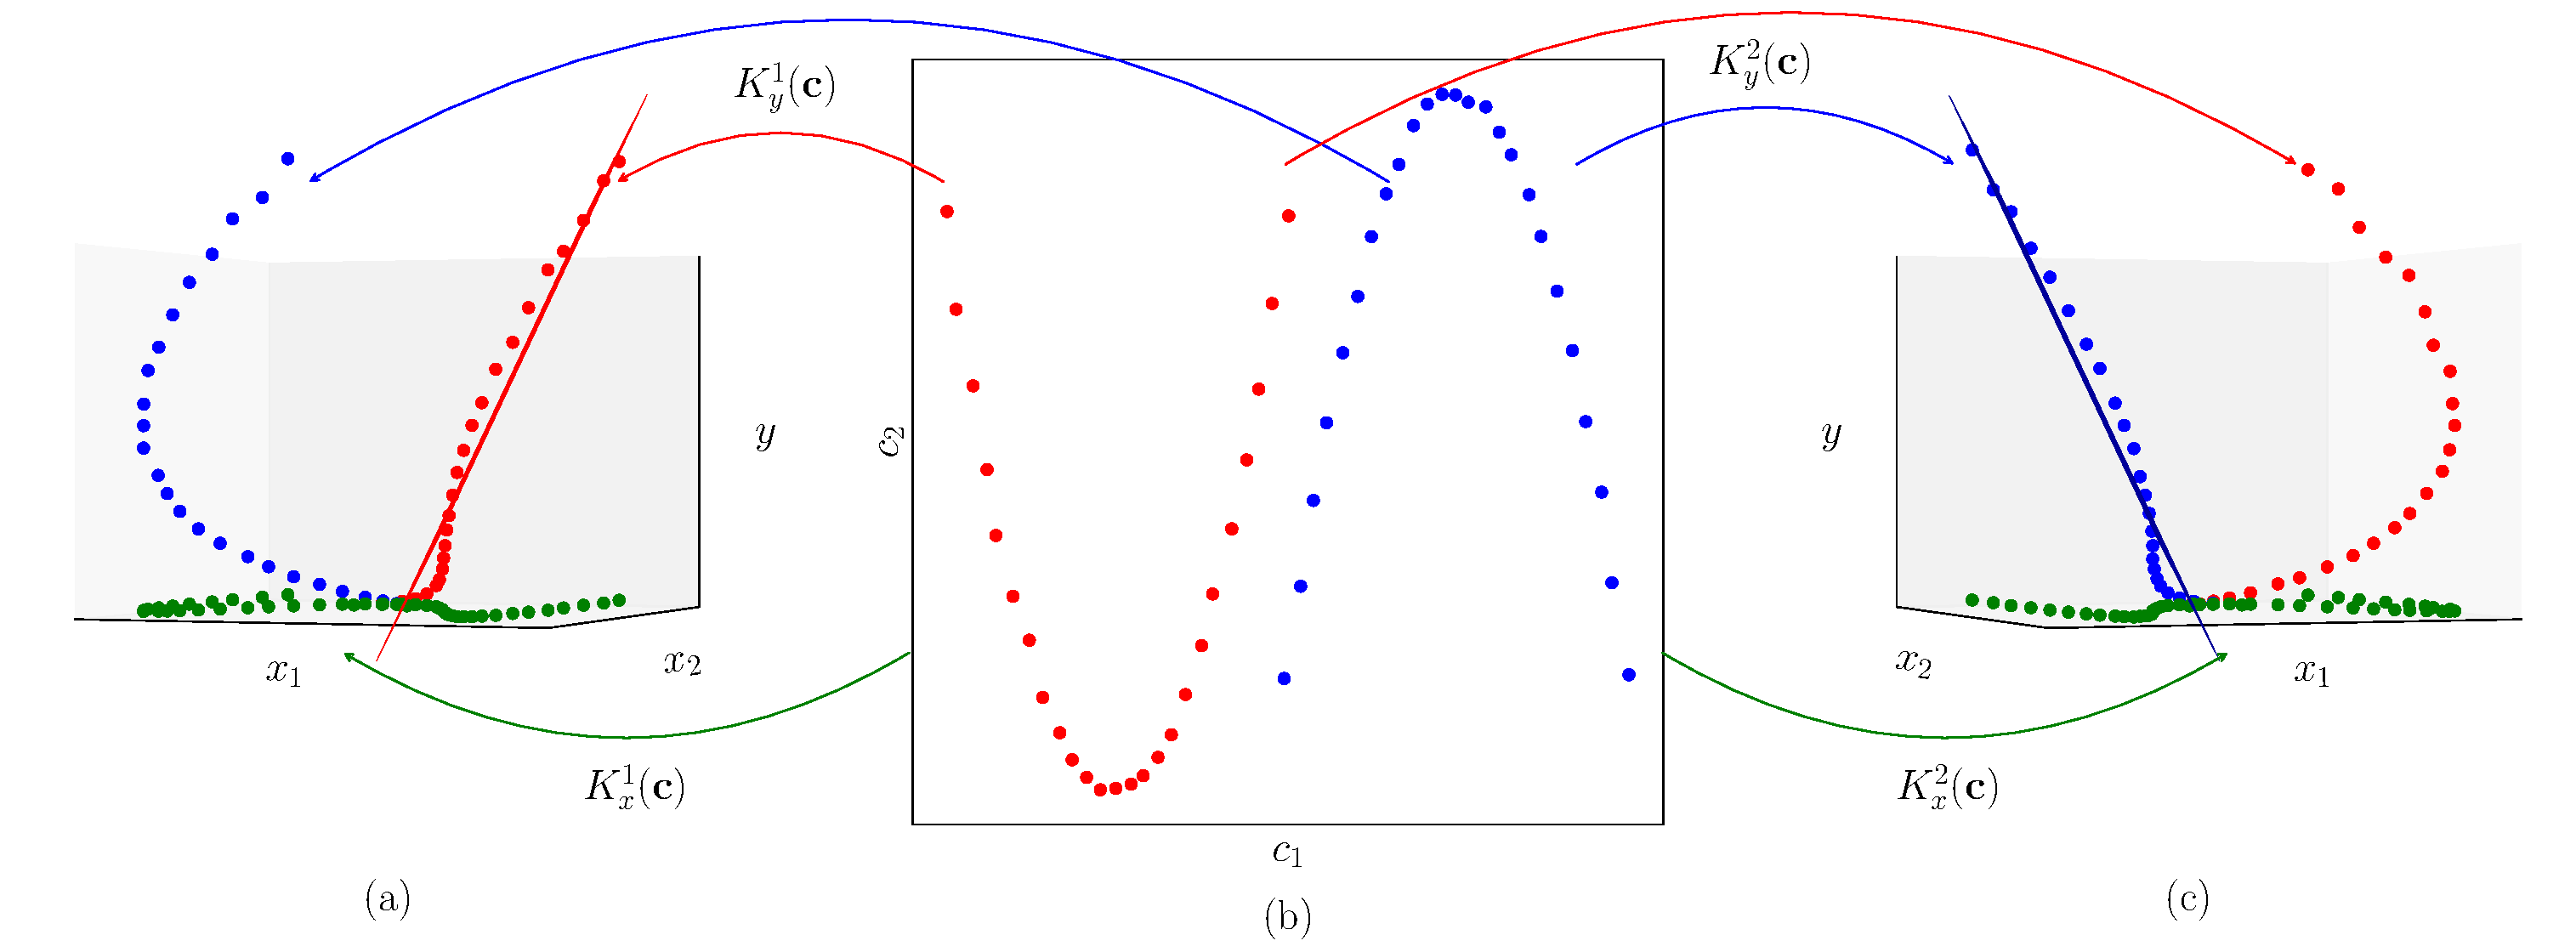
\includegraphics[width=\textwidth]{results/priorexpertfig/explanation}
     \caption{Пример: а) экспертная информация первого эксперта; б) исходные данные; в) экспертная информация второго эксперта}
    \label{intro:fig2}
\end{figure}
На рисунке \ref{intro:fig2} показан пример кривых второго порядка, а также экспертная информация о кривых. На рисунке \ref{intro:fig2}.a показана экспертная информация первого эксперта. Используя эту информацию, первая кривая аппроксимируется линейной моделью, а вторая кривая - шумом. На рисунке \ref{intro:fig2}.b показана экспертная информация второго эксперта. Используя эту информацию, вторая кривая аппроксимируется линейной моделью, а первая кривая представляет собой шум.

При аппроксимации нескольких кривых на одном контурном изображении строится многомодель. Примером нескольких моделей является случайный лес (Chen et al. 2012), бустинг деревьев (Chen et al. 2016), смесь экспертов (Yuksel et al. 2012). В данной работе смесь экспертов рассматривается как мультимодель. Смесь экспертов - это мультимодель, которая линейно взвешивает локальные модели, которые аппроксимируют часть выборки. Значения весовых коэффициентов зависят от объекта, для которого делается прогноз. Для решения проблемы смеси  экспертов используется вариационный EM-алгоритм (Dempster et al. 1997; Bishop 2010; Peng et al. 1996). Смесь экспертов имеет множество применений в ряде приложений. В работе  (Estabrooks et al. 2001) решается задача классификации текстов. В работах (Cheung et al. 1995; Weigend et al. 2000; Cao 2003; Mossavat et al. 2010; Sminchisescu C et al. 2007; Tuerk 2001; Yumlu et al. 2003), используется смесь экспертов для прогнозировать временные ряды для распознавания речи, повседневной деятельности человека и прогнозирования стоимости ценных бумаг. В работе (Ebrahimpour et al. 2009) смесь экспертов рассмотрена для решения задачи распознавания рукописных чисел на изображениях.

В качестве примера рассматривается задача аппроксимации изображения радужной оболочки глаза. На рисунке \ref{intro:fig1:real} показан пример изображения, которое необходимо аппроксимировать. Рассматриваем обработанное изображение, которое дано в виде схемы, пример такого изображения показан на рисунке \ref{intro:fig1:outer}. На рисунке \ref{intro:fig1:outer} показаны две модели окружностей, которые аппроксимируют радужную оболочку глаза. Окружности - простой пример кривой второго порядка.

\begin{figure}[h!]
\center
	\subfloat[]{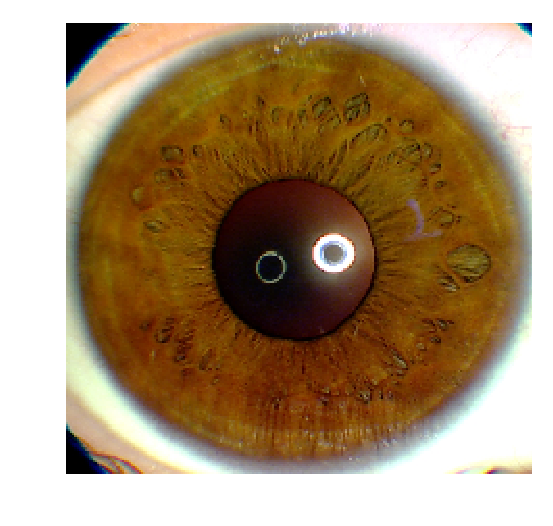
\includegraphics[height = 0.2\textheight]{results/priorexpertfig/real_image}\label{intro:fig1:real}} 
	\subfloat[]{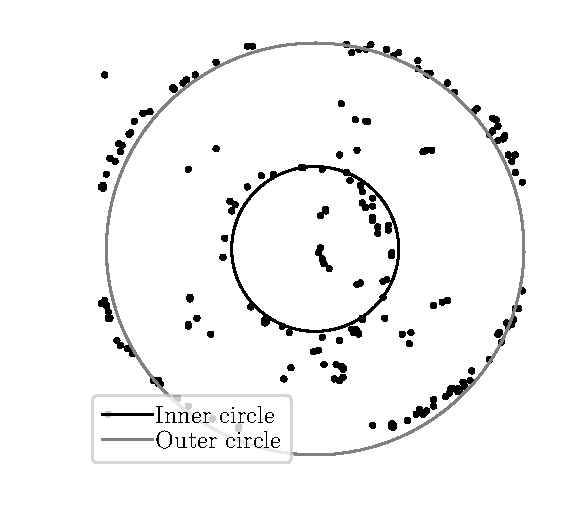
\includegraphics[height = 0.2\textheight]{results/priorexpertfig/outline_image}\label{intro:fig1:outer}} 
\caption{Пример изображения радужной оболочки глаза и ее контурное изображение: а) изображение радужной оболочки глаза; б) контурное изображение радужной оболочки и аппроксимация заданного изображения окружностей}
\label{intro:fig1}
\end{figure}

Для задачи аппроксимации радужной оболочки глаза используется следующая экспертная информация: радужная оболочка глаза аппроксимируется двумя концентрическими окружностями. Экспертная информация используется для построения описания характеристик точек на плоскости, а также для построения функции оптимизации. Часть функции ошибок для оптимизации, использующая экспертную информацию, называется регуляризатором. Таким образом, информация о том, что изображение окружностей задается описанием признака, и информация о том, что концентрические окружности задаются с помощью специального регуляризатора.

В вычислительном эксперименте качество аппроксимации контурного изображения анализируется в зависимости от заданной экспертной информации и от уровня шума в синтетически сгенерированных данных. Анализ качества аппроксимации диафрагмы проводится в зависимости от количества экспертной информации, которая использовалась при построении модели. Обратите внимание, что каждое приблизительное изображение представляет собой отдельный набор точек, которые необходимо приблизить.

